\documentclass{comjnl}

\usepackage{amsmath}
\graphicspath{{images/}}
\usepackage[utf8x]{inputenc}
\usepackage{amsmath}
\usepackage{graphicx}
\usepackage{parskip}
\usepackage{fancyhdr}
\usepackage{vmargin}
%% These two lines are needed to get the correct paper size
%% in TeX Live 2016
\let\pdfpageheight\paperheight
\let\pdfpagewidth\paperwidth

%\copyrightyear{2009} \vol{00} \issue{0} \DOI{000}

\begin{document}

\title[ARTICULO DE INVESTIGACION]{DISMINUCIÓN DE LOS TIEMPOS EN EL REGISTRO DE UN CLIENTE DE UN HOTEL DE LA ZONA HOTELERA DEL MUNICIPIO DE ESCÁRCEGA, CAMPECHE A TRAVÉS DE LA IMPLEMENTACIÓN DE UN SOFTWARE DE CONTROL DE REGISTRO. }

\author{Antonio Mora Navarro}
\email{mora.portador@gmail.com}

\shortauthors{A. Mora}
 
\received{03 Junio 2017}
\revised{12 Junio 2017}



\keywords{Palabras clave: registro, sistemas de registro, impacto, beneficio, factibilidad, hipótesis}


\begin{abstract}
The present document details the development and evaluation of the System of Guest's Record and Inventor control Sale. The system is developed for the company Hotel Akimpech, located in the Av. Solidarity Not. 43 x 45 of the city of Escárcega, Campeche. The aim of this project is to offer a solution to the problem originated in the receipt of the hotel by means of the generation of an IT system that rests on the management of the business, in which 3 variables were in use, such as, to improve the service to the client, to avoid the loss of time of more realizing a search of some record and to measure the times in which they are late in registering a client in the hotels of the region with and without the utilization of the software. In the stage of development of the System of Guest's Record and Inventor control Sale. For the process of development tools were in use adapted to gather necessary information, such as surveys, to know the opinion of the clients on having implemented programs of calculation, to carry out his request of revenue to the hotel. As well as a guide of observation to monitor his attitudes of them to the moment of the record, and after this, implemented a program of record version thread to carry out a comparison to the system of record that nowadays counts the Hotel Akimpech, announcing his advantages and disadvantages of his application to the place.\\


\end{abstract}

\begin{abstract}
El presente documento detalla el desarrollo y evaluación del Sistema de Registro de Huésped y Control de Inventario Venta. El sistema es desarrollado para la empresa Hotel Akimpech, ubicado en la Av. Solidaridad No. 43 x 45 de la ciudad de Escárcega, Campeche. El objetivo de este proyecto es brindar una solución al problema originado en la recepción del hotel mediante la generación de un sistema informático que apoye en la gestión del negocio, en el cual se utilizaron 3 variables, tales como, mejorar el servicio al cliente, evitar la pérdida de tiempo de más realizando una búsqueda de algún registro y medir los tiempos en que se tardan en registrar a un cliente en los hoteles de la región con y sin la utilización del software. En la etapa de desarrollo del Sistema de Registro de Huésped y Control de Inventario Venta. Para el proceso de desarrollo se utilizaron herramientas adecuados para recolectar información necesaria, tales como encuestas, para saber la opinión de los clientes al implementar programas de cómputo, para llevar a cabo su solicitud de ingreso al hotel. Así como una guía de observación para monitorear sus actitudes de ellos al momento del registro, y después de esto, se implementó un programa de registro versión beta para llevar a cabo una comparación al sistema de registro que actualmente cuenta el Hotel Akimpech, dando a conocer sus ventajas y desventajas de su aplicación al local. \\


\end{abstract}

\maketitle


\section{Introduccion}

IMPLEMENTACIÓN DE NUEVAS TENDENCIAS
A medida que la ciudad se moderniza, la población experimenta transformaciones en los estilos de vida, Es por eso que es de suma importancia modernizarse para permitir un mejor desempeño y así tomar ventaja de los demás participantes del rubro. Debido a lo anterior, el hotel AKIMPECH decidió implementar el sistema que permitiría facilitar las labores de los trabajadores enfocándose solamente al servicio prestado. Además, el sistema tiene la posibilidad de mostrar toda la información relacionada con las ventas, desde distintos puntos de vista para la gerencia de la empresa, lo que permite establecer puntos de decisiones con bases sólidas.
De manera en que los años van pasando se va siendo más necesario la implementación de nuevas tendencias para facilitar el trabajo que realiza un recepcionista en un hotel implementando software que le ayuden a el registro para tener un control completo del hotel y no solamente para esto si no para brindar un gran impacto al cliente al momento de llegar a nuestro establecimiento. “Un programa de gestión hotelera es hoy en día fundamental para cubrir las necesidades diarias de cualquier establecimiento turístico que quiera estar a la vanguardia. Automatización, agilización de procesos y centralización de la información, cuya consecuencia inmediata es una clara mejora de la productividad. Así se optimizan y se resuelven rápidamente las funciones operativas, administrativas o de mantenimiento.”
La automatización de procesos es uno de los factores que hacen fundamental la instalación de un programa de gestión hotelera. Operaciones como la generación, gestión y envío de facturas, que normalmente ocupan mucho tiempo y conllevan un gran esfuerzo, se realizan de forma cómoda, con un gran ahorro de costes y con la segura satisfacción del cliente, cuya reserva se gestionará de forma eficaz. (Cloud Computing para Negocio y CEO's, 11/04/2015)
Moreno, 2002, afirma que todas aquellas empresas para las cuales la gestión de la información es una prioridad, como es el casos de las empresas turísticas, utilizan como mínimo un ordenador y otros elementos tecnológicos ya que, cada vez en mayor medida, el método más económico de procesar información en un tiempo oportuno y con calidad suficiente, es la tecnología, y más en concreto las Tecnologías de la Información y la Comunicación.
Con respecto a las TIC y el sector turístico, se cita textualmente: “The tourism system is inevitably influenced by the new business environment created by the diffusion of ICTs. Information technology is one of the external environment elements for tourism, travel and hospitality, although in recent years technological developments have supported tourism innovation and vice versa. ICTs have become an imperative partner, increasingly offering the interface between consumers and suppliers globally.” (Arturo García¬ Santillán, 2011). Es decir que el turismo esta significativamente influenciado por el nuevo entorno comercial creado a partir de la difusión de las TIC, mismas que se han convertido en uno de los elementos del entorno del turismo, viajes y la hospitalidad, aunque en los últimos años los avances tecnológicos han apoyado con su innovación al turismo, también el turismo ha favorecido esta innovación, al demandar aspectos específicos que la tecnología debe satisfacer. Concluye diciendo que las TIC se han convertido en un socio indispensable, ofreciendo cada vez más la interfaz entre consumidores y proveedores a nivel mundial.
El problema se presenta en los proceso de reserva, registro y facturación del huésped. Todo sucede cuando el posible huésped llama al hotel y se le toman los datos personales necesarios para validar la reserva. Este se guarda en un formato de papel y es archivado en un sección en donde se encuentran todas las reservas realizadas por que el sistema actual es incapaz de guardarlo, El
proceso de registro se ejecuta de la siguiente manera; se ejecutan los datos del huésped y se confirma la reserva, pero como el sistema presenta dificultad para guardar dicha información, cuando éste se cierra, esta información desaparece, trayendo como consecuencia la pérdida del cliente, porque cuando este llega al hotel al no aparecer la reservación se disgusta por que la habitación aparece ocupada por otra persona. 
Otra dificultad que se presenta en la facturación es que el sistema no registra el consumo que hace el cliente por tanto este proceso es llevado manualmente, muchas veces este registro no se hace adecuadamente lo que conlleva a que cuando el cliente pide su factura para cancelar no existe un registro detallado de lo que ha consumido y el cliente tiene que informar lo consumido durante su estadía. En esta situación se corre el riesgo de que el cliente dé una información errada y el hotel registren pérdidas por falta de registro oportuno de la información.


\section{Marco de desarrollo} \label{Model}
En el presente trabajo se tomó en cuenta la tabla de comparación, el cual se consideró para recolectar los datos de los tiempos, de igual forma se realizó la elaboración del plan de evaluación de desempeño al personal del Hotel Akimpech. 
Se realizó un formulario de preguntas de satisfacción del uso del software para el cliente y para el recepcionista, esto con la finalidad de realizar la formulación de un algoritmo para realizar la comparación.




\section{Hipótesis} \label{Model}

•	El manejo y uso del software de control de registro mejorara el rendimiento de registro que realiza el recepcionista.
•	El manejo del software reducirá el tiempo en la búsqueda de algún registro que se desee buscar en el momento.

\newpage

\section{Resultados Importantes}
El coeficiente de correlación de Pearson, que se simboliza con la letra minúscula r, se
calcula dividiendo la suma de los productos de las desviaciones de cada variante de X
e Y, con respecto a sus medias (suma que se denomina covarianza de X e Y), por el
producto de las desviaciones estándar de ambas variables. En forma práctica, el
coeficiente de correlación de Pearson es: 
\begin{figure}[!htb]
En las imágenes que ahora veremos corrresponderan a las correlaciones de datos menores y mayores, no sin antes mostrar la fórmula utilizada.
\centering
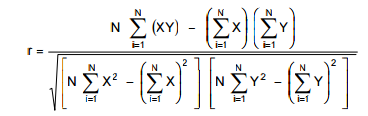
\includegraphics 
[scale=.7]{per.PNG}
\caption{COEFICIENTE DE CORRELACIÓN }
\end{figure}
donde N es el número de datos.
\begin{figure}[!htb]
La siguiente tabla demuestra la informacion recolectada con los metodos de recoleccion de datos, dicha información fue obtenida aplicando encuestas y el metodo de observación. Aplicadas estratégicamente en la zona hotelera de la región.
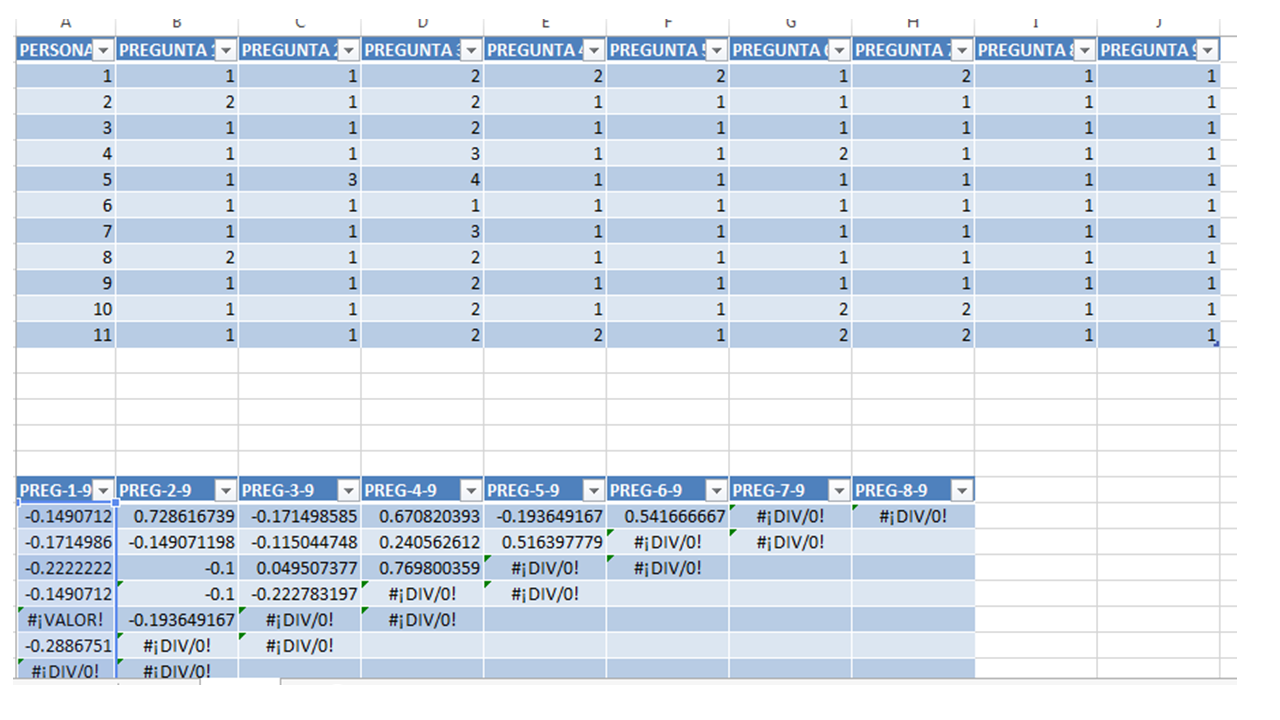
\includegraphics 
[scale=.3]{Presentaci_n45.png}
\end{figure}\\
Con anterior significa que, entre 0 y +1 cabe toda una gama de correlaciones positivas,
que serán tanto más directamente proporcionales, cuanto más se acerquen a +1.
Similarmente entre –1 y 0 cabe toda una gama de correlaciones negativas, que serán
tanto más inversamente proporcionales, cuanto más se acerquen a –1. Los
coeficientes de correlación, cuanto más cerca de cero, indican menor correlación. 
\\
Por lo tanto en las imagenes de abajo se podrán ver las correlaciones generadas con los resultados obtenidos en la tabla de arriba.
\begin{figure}[!htb]
En esta imagen se puede observar una gráfica correspondientes a las correlaciones mayores existes en todos los datos, existe una correlación entre ellas debido a que los datos estadísticos no varían en su escala de medición.
El coeficiente de correlación lineal es un número real comprendido entre menos −1 y 1.
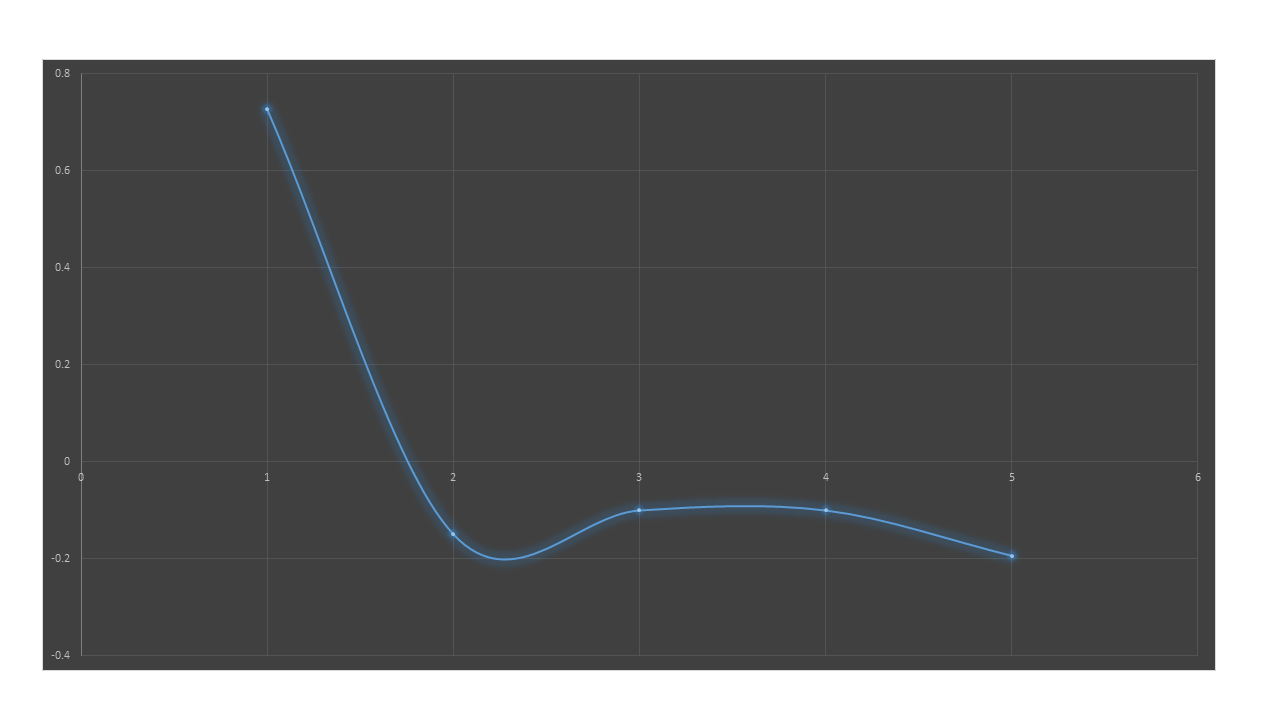
\includegraphics 
[scale=.2]{Diapositiva1.PNG}
\end{figure}\\

\begin{figure}[!htb]
En las imágenes que ahora veremos corrresponderan a las correlaciones de datos menores, esto debido a que  toma valores cercanos a 0 y la correlación es débil.
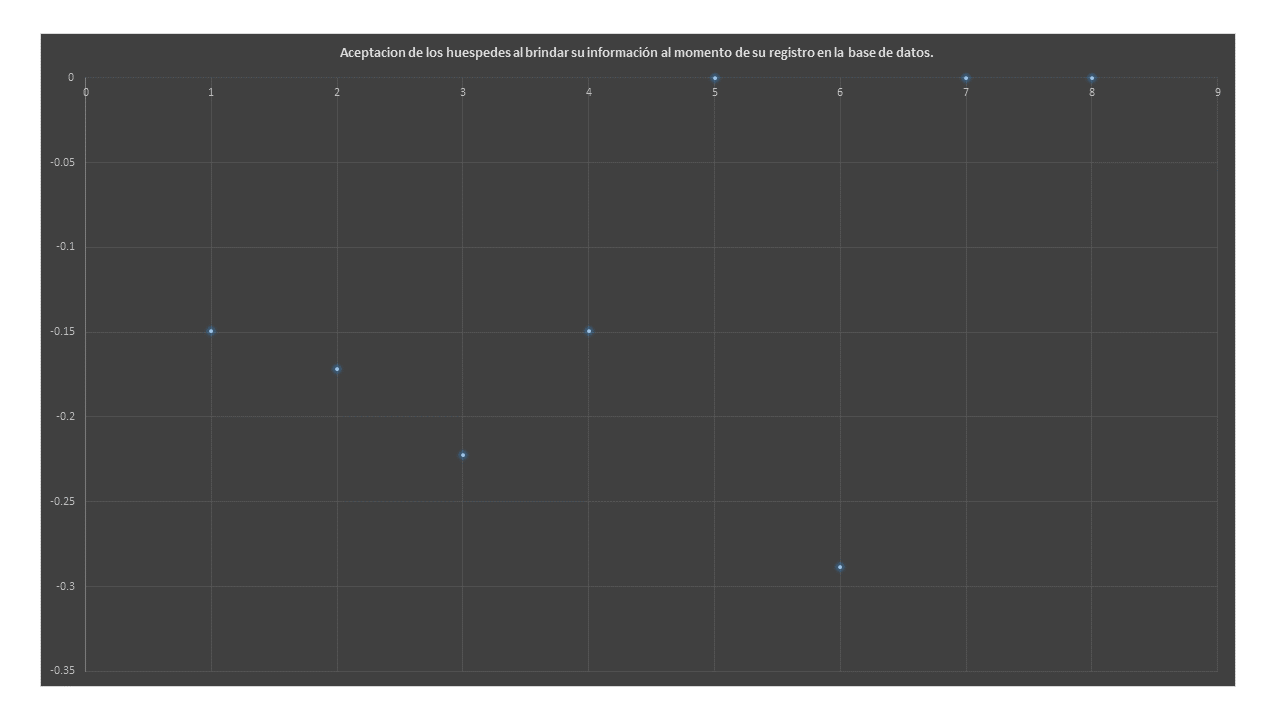
\includegraphics 
[scale=.2]{Diapositiva2.PNG}
\end{figure}

\newpage
\section{Conclusión }
Los sistemas informáticos tienen grandes ventajas en diferentes áreas de trabajo, un ejemplo claro, es en el registro de un cliente de un hotel en el municipio de Escárcega, Campeche, ya que con estos sistemas se disminuyen tiempos y se ahorra papelería. 
Se aplicaron encuestas para saber la opinión de los clientes al implementar programas de cómputo, para llevar a cabo su solicitud de ingreso al hotel, así como una guía de observación para monitorear sus actitudes de ellos al momento del registro, dando como resultado una buena aceptación por parte de los clientes.

\nocite{*}
\section{Referencias}
\bibliographystyle{compj}
\bibliography{ModellingBidders}
Arturo García¬Santillán, M. C. (2011). LOS SISTEMAS INFORMÁTICOS DE GESTIÓN HOTELERA Y LOS BENEFICIOS DE SU IMPLEMENTACIÓN. TURyDES.
Cloud Computing para Negocio y CEO's, C. R. (11/04/2015). ¿Por qué utilizar un programa de gestión hotelera? Cloud Computing para Negocio y CEO's, Cloud Retail, 7.
Moreno, R. (2002). Rufin Moreno. Rufin Moreno.



\end{document}